
\chapter{Background}

\section{Introduction}

This research builds on two existing paradigms in software development: reactive programming and the dataflow model. While intimate knowledge about these concepts is not required, a basic understanding of both will be necessary to follow the ideas and implementation of this dissertation. Reactive Programming is situated in the category of higher level software development, serving as an abstraction tool for events and reactions to those events. The dataflow model on the other hand can be considered more 'low level', providing a strategy for the implicitly parallel execution of programs. 

\newpage

\section{Reactive Programming}

Reactive Programming is a software development paradigm focused on reactions, i.e. the handling of external events, user interactions, etc.  In this paradigm, the application state is derived from the previous state and any events that may occur, for example user interactions or current environmental factors. This deviates from more traditional approaches, where values and state can be written at any point and for any reason. In a reactive program however, the flow of dependencies is recorded as a (possibly cyclic!) directed graph, making the derivation of the application state very explicit.
At the core of reactive programming are the following main concepts:
\begin{itemize}
	\item The first-class reification of events (making events a first-class citizen)
	\item The composition of these events through lifted functions
	\item The automatic tracking of dependencies and re-evaluation by the language runtime
\end{itemize}

A number of implementations exist for reactive programming, in this thesis we will focus on the interpretation taken in FrTime. 

\subsection{Example}

The canonical metaphor for Reactive Programming is spreadsheets, which typically track changes across input cells and automatically recompute values in other cells if the formulas they contain reference the aforementioned input cells. In essence, cells react to modifications made in other cells if their formulas depend on them. These cells are what we call \textit{observables} or \textit{signals} in Reactive Programming.
Imagine a simple program in an imperative programming setting:

\begin{lstlisting}
	a = b + c
\end{lstlisting}

When this statement is executed, it assigns the result of adding b and c to the variable a, mutating a in the current scope. Note that this only happens once. A snapshot is taken of the current value of b and c, to determine the new value of variable a. Of course, this assumes that the variable b and c are provided to the program.

\begin{figure}[h]
	\centering{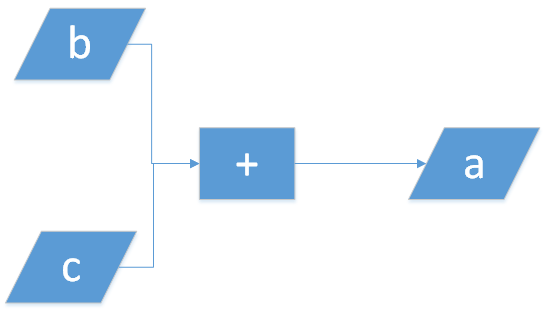
\includegraphics[width=\textwidth]{images/background-reactive-example.png}}
	\caption{Graph of signals}
	\label{fig:background-reactive-example}
\end{figure}

In a reactive programming setting, a would subscribe to the values of b and c, essentially asking to be notified whenever the variables b or c change, at which point the value of variable a changes. See figure \ref{fig:background-reactive-example} for the reactive graph. This process repeats every time the variables b or c are modified. Note that the value of a is undetermined until both b and c produce a value. 

The implementation of this reactive mechanism can be provided by the language itself or by a framework or library. 

\subsection{Advantages of Reactive Programming}

A signal can be described as "values over time", in contrast with a variable which only holds its latest value, revealing no information about the time that value was provided or what changed it. 
Signals can be used to model almost any concept in software development:
\begin{itemize}
	\item mouse movements as a signal which emits the current position in real time
	\item click events as a signal which emits event objects
	\item the results of a database query as a signal which emits only one value
    \item an infinite sequence as a signal which never stops emitting
\end{itemize}

Even though the underlying mechanism will still be identical to more traditional approaches (attaching event listeners to DOM events in HTML, opening and connecting to a WebSocket connection, etc.), the fact that all these concepts can be brought together under a single umbrella called \textit{signals} allows for the modeling of higher order operators to map, combine and filter these flows of values in ways that were previously a lot harder.

\section{The Dataflow Model}

\subsection{Introduction}

The dataflow model is a paradigm focused on the parallel execution of programs. In this paradigm, instructions are seen as isolated units, which should be able to execute whenever the necessary parameters have been provided. Contrary to imperative programming, instructions are not invoked by a program counter, but rather whenever all of the parameters are present. 

The execution of instructions in the dataflow model can be seen as a direct graph of nodes where each node represents an instruction and each edge is the output being sent to the next instructions that require the output as arguments. It is up to the dataflow engine to orchestrate the flow of arguments so that instructions are invoked correctly and in the correct order.

Whenever an instruction is invoked, the output is sent through to all connected instructions which depend on it. In Tagged Token Dataflow systems, instruction arguments are wrapped in tokens, which carry meta data about which execution context they belong to in order to isolate multiple calls to the same instruction from one another.

A large difference with Reactive Programming is that Dataflow Programming puts the instruction invocation at the center stage, while Reactive Programming puts forward signals as the core concept of its paradigm. In other words, while both systems have the notion of a dependency graph, the nodes in their graphs carry different concepts: instructions and signals respectively.
 
\newpage

\subsection{Example}

Imagine a simple program in an imperative programming setting:

\begin{lstlisting}
a = b + c
d = a + b
\end{lstlisting}

This assumes that the variable b and c are provided to the program.
In a traditional execution, the variable a would be set to the sum of b and c and the variable d would be set to the sum of a and b. Note that the sequence in which these operations are executed is of vital importance: switching the two statements would result in different values for the variable d!

\begin{figure}[h]
    \centerline{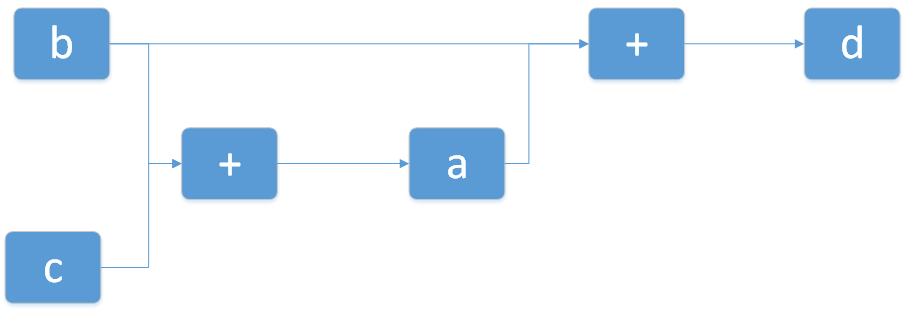
\includegraphics[width=\textwidth]{images/background-dataflow-example.png}}
	\caption{Graph of instructions}
	\label{fig:background-dataflow-example}
\end{figure}

In a dataflow engine, these instructions would be registered as instructions in the dependency graph, as visualized by figure \ref{fig:background-dataflow-example}. The values of b and c would be added to the queue at application startup. B would be entered as a token twice; once for the instruction "+" which computes a and once for the instruction "+" which computes d. When the dataflow engine spins up and starts processing arguments, it sends the tokens for b and c to the first "+" instruction, which is triggered because all of its inputs are present and valid. This produces a value for variable a, which gets added to the token queue again as the first parameter for the second "+" instruction. This instruction now also has all of its inputs present, which allows it to compute the value for variable d at this point.

If at any point in the future, b or c (which should be seen as the output of other instructions not shown in the sample code) produce new values, these would be enqueued again for further processing.

\subsection{Advantages}

The key advantage of the data flow model is that only the data dependencies of the instructions decide when an instruction can be executed. Since data flow instructions are not allowed to access or manipulate shared state, each instruction is completely isolated. This means that all dataflow instructions can be run in parallel, across different processes and even separate machines.

\section{Conclusion}

Two paradigms were presented: reactive programming and the dataflow model. 
Reactive programming is targeted more towards events and reactions and shines best in environments where these things are plenty, for example in user interfaces and other places where events can come from any direction. The dataflow model on its part focuses more on the parallel execution of instructions by streaming parameters to them in isolated scopes. We do however note similarities between the two, namely that they both work with an update graph that guides the data along the nodes. 



